% Author: Till Tantau
% Source: The PGF/TikZ manual
\documentclass[a4paper,11pt]{article}
\usepackage[utf8]{inputenc}
\usepackage{listings}
\usepackage{amsmath}    % need for subequations
\usepackage{graphicx}   % need for figures
\usepackage{verbatim}   % useful for program listings
\usepackage{color}      % use if color is used in text
%\usepackage{subfigure}  % use for side-by-side figures
\usepackage{hyperref}   % use for hypertext links, including those to external documents and URLs
\usepackage{url}
\usepackage{float}
\usepackage{tikz}
\usepackage{enumitem}
\usepackage{hyperref}
\usepackage{pdfpages}
\usepackage{caption}
\usepackage{subcaption}
\usepackage{listings}
\usepackage{color}
\usepackage{amsfonts}
\usepackage{latexsym}
\usepackage[T1]{fontenc} % use for allowing < and > in cleartext
\usepackage{fixltx2e}    % use for textsubscript
\usepackage[linesnumbered,boxed,ruled]{algorithm2e}
\newcommand{\BigO}[1]{\ensuremath{\operatorname{O}\left(#1\right)}}
\definecolor{mygreen}{rgb}{0,0.6,0}
\definecolor{mygray}{rgb}{0.5,0.5,0.5}
\definecolor{mymauve}{rgb}{0.58,0,0.82}
\lstset{ %
  backgroundcolor=\color{white},   % choose the background color; you must add \usepackage{color} or \usepackage{xcolor}
  basicstyle=\footnotesize,        % the size of the fonts that are used for the code
  breakatwhitespace=false,         % sets if automatic breaks should only happen at whitespace
  breaklines=true,                 % sets automatic line breaking
  captionpos=b,                    % sets the caption-position to bottom
  commentstyle=\color{mygreen},    % comment style
  deletekeywords={...},            % if you want to delete keywords from the given language
  escapeinside={\%*}{*)},          % if you want to add LaTeX within your code
  extendedchars=true,              % lets you use non-ASCII characters; for 8-bits encodings only, does not work with UTF-8
  %frame=single,                    % adds a frame around the code
  keepspaces=true,                 % keeps spaces in text, useful for keeping indentation of code (possibly needs columns=flexible)
  keywordstyle=\color{blue},       % keyword style
  language=Octave,                 % the language of the code
  morekeywords={*,...},            % if you want to add more keywords to the set
  numbers=left,                    % where to put the line-numbers; possible values are (none, left, right)
  numbersep=5pt,                   % how far the line-numbers are from the code
  numberstyle=\tiny\color{mygray}, % the style that is used for the line-numbers
  rulecolor=\color{black},         % if not set, the frame-color may be changed on line-breaks within not-black text (e.g. comments (green here))
  showspaces=false,                % show spaces everywhere adding particular underscores; it overrides 'showstringspaces'
  showstringspaces=false,          % underline spaces within strings only
  showtabs=false,                  % show tabs within strings adding particular underscores
  stepnumber=2,                    % the step between two line-numbers. If it's 1, each line will be numbered
  stringstyle=\color{mymauve},     % string literal style
  tabsize=2,                       % sets default tabsize to 2 spaces
  %title=\lstname                   % show the filename of files included with \lstinputlisting; also try caption instead of title
}

\bibliographystyle{plain}
\begin{document}
\date{1. December 2013}
\title{Finding Hollywood's most Popular\\Using Map-Reduce and Approximation}

\author{Marcus Gregersen\and Martin Faartoft\and Rick Marker}
%Overkill med forside / abstract / titel / undertitel?
\clearpage\maketitle
\thispagestyle{empty}
\setcounter{page}{1}
\section{The "Popular" problem}
\subsection{Introduction}
In this section, we try to answer the question: "How many unique co-actors has a a given actor starred alongside", we call this the \emph{Popular} problem. In the following, we will develop and execute a Map-Reduce algorithm using the Hadoop framework, both locally and on the Amazon Elastic Cloud service.
\paragraph{}
To validate and compare the Map-Reduce implementation, we will implement a simple, sequential algorithm that solves the same problem. In order to make the problem harder, we have converted the IMDB dataset to a format that forces the Map-Reduce algorithm to use 2 rounds of computation.
\paragraph{} 
To allow for comparison between the sequential and the Map-Reduce algorithms, we have made the sequential algorithm accept the same input.
%TODO skriv noget om problem size, antal actors, antal movies, textfil størrelse
\subsection{Naïve Sequential Algorithm}
\label{sub:sequential}
%TODO reference for inverted index
In the sequential algorithm we build an inverted index, that maps movies to the actors that star in them. This allows us to check which actors appear in which film in constant time. Building the index takes \BigO{a*m} time, where \emph{a} is the number of actors and \emph{m} is the number of movies\\

When the inverted index is built, we iterate over all actors in the dataset, and for each actor we iterate over the movies they appear in, and for each of those, we note their co-actors. For each co-actor a given actor has starred with we add it to that actors total. Even though all lookups are implemented to be done in constant time, having 3 nested loops, we get a running time of \BigO{a^2*m}. Finally we write the output, which takes another \BigO{a*m} time.\\

This gives our sequential algorithm a worst-case running time of \BigO{a^2*m}. When running the algorithm on the dataset, the actual running time is much better than the theoretical worst-case. If we envision a matrix with actors and movies, where each entry is 1 if the actor appeared in the movie, or empty otherwise, we can see that the matrix is pretty sparse with the given IMDB dataset. As a result the actual running time of our algorithm will be much lower.

\subsection{Map-Reduce Algorithm}
\label{sub:map-reduce}
\begin{figure}
\centering 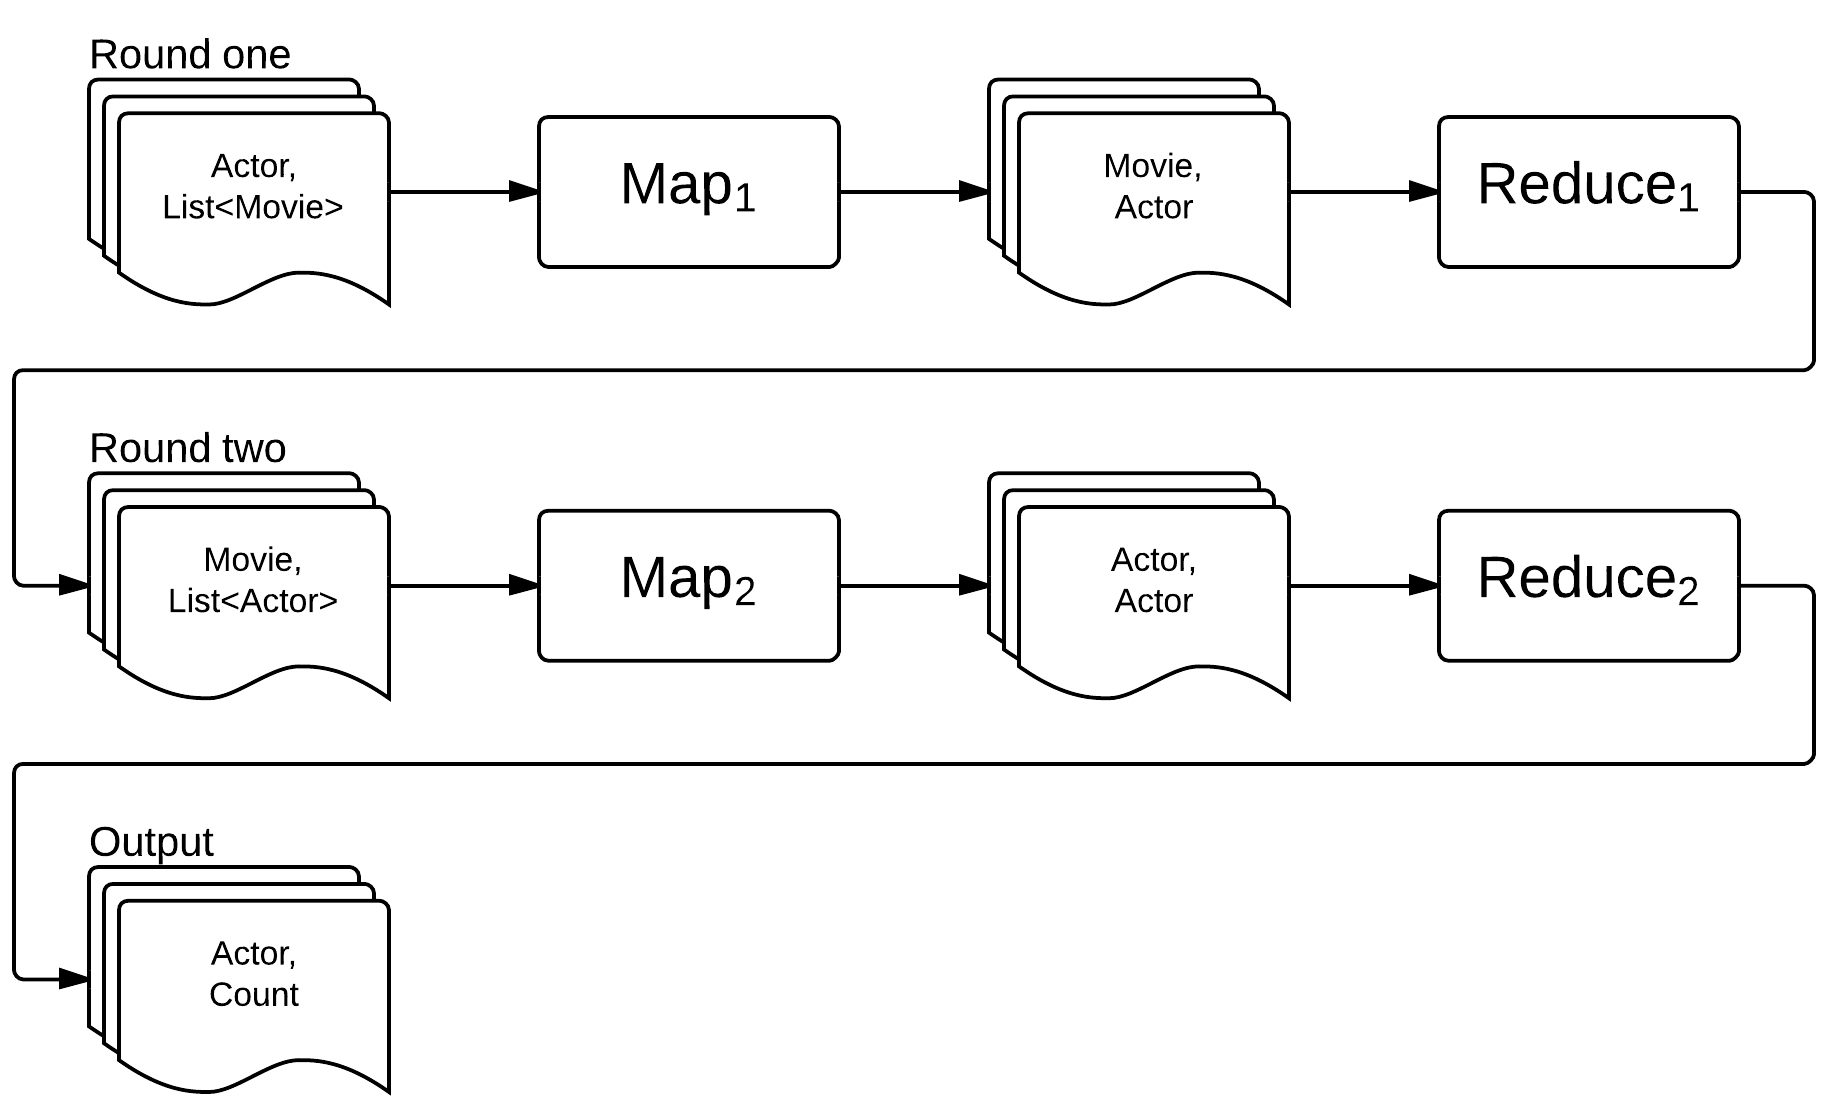
\includegraphics[scale=0.2]{map-reduce-figure.png}
\vspace{-10pt}
\caption{Map-Reduce overview}
\label{fig:map-reduce}
\vspace{-10pt}
\end{figure}

Solving the \emph{Popular} problem using Map-Reduce with the specified input format, requires two rounds. The first round will pivot the input into a more suitable structure, while the second round will answer the actual question, that is count the number of unique pairings of actors.

\subsubsection{Round One}
Goal: Transform input pairs (Actor, List<Movie>) into output pairs (Movie, List<Actor>).\\

The mappers break down the (Actor, List<Movie>) pairs into a series of (Movie, Actor) pairs, one for each Movie in the input List<Movie>, essentially emitting the information: "this actor played in this movie".\\

The shuffle step (part of the Hadoop framework), directs each pair emitted by a mapper, to a reducer, such that every pair with a given key k, is sent as input to a single reducer R\textsubscript{k}.\\

The reducers each receive a list of (Movie, Actor) pairs, and builds from those a single pair (Movie, List<Actor>) by simply appending each actor to a list. The output of round one is thus, a pivot of the input data changing the shape from (Actor, List<Movie>) to (Movie, List<Actor>), essentially saying "this movie contained exactly these actors".

\subsubsection{Round Two}
\label{sub}
Goal: Transform input pairs (Movie, List<Actor>) into output pairs (Actor, Count), where count is the number of unique co-actors this actor has starred with in a movie.\\

The mappers break down the (Movie, List<Actor>) pairs into all possible Actor-pairs along with their inverses.

\begin{verbatim}
function RoundTwoMap(...)
    for(actor a in actors)
        for(actor b in actors)
            if(a != b)
                emit(a, b)
\end{verbatim}

This produces a number of pairs, quadratic in the number of actors in the movie, each capturing the information "Actor A played with Actor B in some movie".\\

The reducers each receive a list of (Actor\textsubscript{key}, Actor\textsubscript{value}) pairs, and using a Java HashSet\footnote{The 'Set' interface guarantees that no two equal objects can be contained in the set, at the same time.}, they filter out any duplicate pairs, and emit the final (Actor, count) pairs, one for each actor. These pairs give the number of unique co-actors, a given actor has had during his career.

\subsubsection{Analysis}
To gauge the efficiency of our implementation, we look at three important performance measures from a Map-Reduce point of view. The number of rounds in the computation, the amount of work done in each mapper/reducer (in the worst case), and the number of pairs emitted.

\paragraph{Number of rounds}
The algorithm runs in a constant number of rounds (2), independent of the problem size. As mentioned previously, this can be reduced to a single round, if the input has a more suitable structure.

\paragraph{Work distribution (skewness)}
The amount of work done in each mapper/reducer is close to being balanced. Obviously, the round two reducer assigned to the most productive actor in the dataset, will do more work than the reducer assigned to an actor that only star in a single movie, but in terms of the input size, these numbers are very close to each other. This is only true because no actor has played in a significant fraction of the total number of movies in the dataset.\footnote{If this was not true, additional techniques, beyond the scope of this project, would be needed to balance the workload.}

\paragraph{Number of pairs}
The number of pairs generated in round two, is proportional to the number of unique pairs of actors that starred in a movie together. For every movie that has A actors starring in it, $2*A(A-1)$ pairs will be emitted. %TODO does this need a further explanation?

This is a large amount of pairs, but we cannot see how this number can be reduced, without relaxing the constraint that a pair of actors should be counted only once. If that constraint is lifted, the round two mapper can simply emit (Actor, Movies.Actors.count - 1), meaning that "this actor starred with n other actors in some movie". The reducers could then simply sum all those counts, to get the total.\footnote{This optimization captures the same idea as the standard 'Wordcount' optimization example, where the mapper keeps a local dictionary of words and counts, instead of mindlessly emitting (word, 1) duplicate pairs multiple times.}\\
% TODO: Should we analyse the other version as an approximation algorithm for the initial problem.
The relaxed version of round two produces drastically fewer pairs (one pair for each actor, for each movie they starred in), compared to the strict version (two pairs for each unique pair of actors per movie). By making the mapper slightly smarter, the shuffler and reducers do much less work. But it also solves a slightly different problem, than the one we are interested in. Overall the performance on the given dataset is acceptable, but for significantly larger datasets, the number of pairs might cause a noticeable slowdown.

\subsection{Verification of results}
We have designed the format of the output of our sequential algorithm, described in Section \ref{sub:sequential}, in such a way that it conforms to the format of the Map-Reduce algorithm described in Section \ref{sub:map-reduce}. 
The output is thus on the form:
\begin{verbatim}
[ 
  (Actor_ID_1, Count_1),
  (Actor_ID_2, Count_2),
  ...
  (Actor_ID_n, Count_n)
]
\end{verbatim}
Since we have no guarantee that the row \texttt{Actor\_ID} is sorted in the output of the Map-Reduce algorithm, we have implemented a simple Python script \texttt{sort\_and\_expand.py}. 
The role of this script is firstly to sort the input by \texttt{Actor\_ID} and secondly to add the first and last name of the actor in question, for more readable output.

Having three different outputs produced by a: the sequential algorithm, b: the Map-Reduce algorithm run on a local machine, and c: the Map-Reduce algorithm run on the Amazon Elastic MapReduce service, we then transform these outputs using the script.
Using the UNIX tool \texttt{diff}, whose job it is to output the difference between two files, we see that that all three outputs are exactly the same.

The fact that two algorithms, developed by different people, using different programming languages and different algorithmic paradigms, produce the same output, gives us a very high confidence in the correctness of both implementations. The odds of introducing the same systematic error into both, are extremely low.

The first 10 lines of the output, i.e the top 10 actors that has starred with most unique actors are: 
\begin{verbatim}
(621468, 'Bess Flowers', 10834)
(372839, 'Lee Phelps', 6679)
(74450, 'John Carradine', 6447)
(212581, 'Stuart Holmes', 6318)
(152868, 'James Flavin', 6027)
(22585, 'Irving Bacon', 5957)
(233082, 'James Earl Jones', 5894)
(245158, 'Donald (I) Kerr', 5775)
(209799, 'Adolf Hitler', 5773)
(433904, 'Martin Sheen', 5764)
\end{verbatim}

Taking one sample from the output we see from Bess Flowers' Wikipedia that she was a Hollywood extra that has appeared in over 700 movies. It seems safe to assume that since she has starred in so many movies she would also be starring with a lot of other actors

We realize that this is not a formal proof that the algorithm produces the correct output.

%MABG
\subsection{Benchmark}
We have carried out a small scale benchmark experiment to test the difference in running time between the sequential and the Map-Reduce algorithms, the latter in both a local and a distributed setup. 

For the local setup we used a 2.5 GHz Intel Core i5 chip (denoted as $Local^*$ in the table). 

In the distributed setup we used the online web service Amazon Elastic Mapreduce that runs a customized version of Hadoop. 

The results of the experiment is seen in Table \ref{tab:benchmark}

\begin{table}[h!]
\label{tab:benchmark}
\begin{center}
    \begin{tabular}{|l|l|l|l|l|}
    \hline
    Type       & Local / Distributed & Instances & Instance type                     & Time (sec) \\ \hline
    Sequential & Local               & 1         & $Local^*$ & 66                 \\ \hline
    Map-Reduce & Local               & 1         & $Local^*$ & 244                 \\ \hline
    Map-Reduce & Distributed         & 2         & m1.small                          & 840                 \\ \hline
    Map-Reduce & Distributed         & 10        & m1.small                          & 600                 \\ \hline
    Map-Reduce & Distributed         & 2         & m1.xlarge                         & 180                 \\ \hline
    Map-Reduce & Distributed         & 10        & m1.xlarge                         & 120                 \\ \hline
    \end{tabular}
    \end{center}
    \caption{The results of our experiment}
\end{table}
Our experiment does not contain enough data to make any sweeping conclusions, but it does illustrate a tendency in the distributed setup that more powerful instances yield a faster running time and more instances yield a faster running time. 

The experiment also shows that the sequential algorithm yields the fastest running time, we have been able to achieve. 
It is our strong belief that if the dataset was larger we would see the distributed setup execute significantly faster than the sequential.

\subsection{Solving the "Popular" problem by approximation}
Computing the exact solution, using our Map-Reduce approach, may not scale well with the size of the input, due to the number of pairs emitted. In the following, we suggest an algorithm for approximating the solution, building on previous results by TODO REF PAGH.

\subsubsection{Equivalence of problems}
The Popular problem can be expressed as a boolean matrix multiplication. Consider a matrix A of size $|actors|*|movies|$, where the value $1$ at position $(x, y)$ means that actor $x$ starred in movie $y$. $R = A * A^T$ will then have the dimensions $|actors|*|actors|$, and a $1$ at position $(x, y)$ indicates that actor $x$ and $y$ starred in at least one movie together. Summing the number of non-zero entries in $R_{i,j}$ for a given $i$, gives the number of unique actors that actor $i$ starred with at least once, which is exactly the value we want to compute.\\
Additionally, matrix multiplication can be expressed as the \emph{join-distinct} operation from relational algebra as follows: Consider the boolean matrix multiplication: $R = A \cdot C$. Let the relation $R_1$ be the pairs corresponding to the non-zero values in A, and the $R_2$ be the pairs corresponding to non-zero values in C. Now each unique pair in $R_1 \Join R_2$ will correspond to a non-zero value in R.


\subsubsection{Related Works}
  %Bar-Yossef og Pagh
    %introduce Amossen algorithm
    %uses bar-yossef idea and clever trick where sorting the hashvalues can allow you to skip checking some of them.

%outline:
  %our twist / what we change in our variant
  %preparation (introduction of variables)
  %pseudocode, done
\subsubsection{Our Algorithm}
To solve our problem we propose a variant of the algorithm shown by Amossen et al. in \cite{paper:Amossen}. Instead of approximating the total number of distinct values $\pi_{ac}(R_1 \Join R_2)$ for $R_1(a,b)$, $R_2(b,c)$, we are interested in estimating the number of distinct values $\pi_{ac}(R_1 \Join R_2)$ for each distinct value of $a$ for $a \subseteq c$.\\ % C subset af a
In regards to the popular problem our algorithm can intuitively does the following steps: We iterate through all our movies. For each movie we use the same approach as in \cite{paper:Amossen} to reduce our work from polynomial time to linear time. Then afterwards we use the approximation technique brought forth by Bar-Yossef et al. in \cite{paper:Bar-Yossef}, to compute our estimates.

\paragraph{Introduction}
To be able to understand the algorithm we introduce the following variables:
\begin{itemize}
  \item $B$: $\pi_{b}(R_1 \cup R_2)$
  \item $A_i$: $\pi_{a}(\sigma_{b=i}(R_1))$
  \item $C_i$: $\pi_{c}(\sigma_{b=i}(R_2))$
  \item $W$: Chosen subset of $\pi_{a}(R_1)$
  \item $k$: Size of sketch
  \item $h_1 : \mathbb{R} \rightarrow [0,1]$
  \item $h_2 : \mathbb{R} \rightarrow [0,1]$
  \item $h : [0,1] \times [0,1] \rightarrow [0,1]$
\end{itemize}
Where $h_1$, $h_2$ and $h$ are pairwise independent.

\paragraph{Approach}
Intuitively we create a table for each value $i \in B$. These tables have the dimension $|A_i\cap W|\cdot | \times |C_i|$, where the rows are sorted according to $h_1$ and the columns are sorted according to $h_2$. Each entry in the table is the computed value of $h$ for the pair. We loop through this 

The algorithm works by creating a hashmap mapping $R_1(c)$ to $R_1(b)$, which can be done in linear time. Then for each key we sort
We start by looking at the distinct values of $\pi_{b}(R_1 \cup R_2)$

In order for our algorithm to work we need three hash functions, $h_1(x)$, $h_2(x)$ and $h(x,y)$ which are pairwise independant and all maps into the range [0,1]. $h_1$ and $h_2$ are chosen at random but $h$ is defined as:
\begin{center}
$h(x,y) = (h_1(x) - h_2(x))$ mod $1$
\end{center}

This is done by first looping through all values in $\pi_{b}(R_1 \cup R_2)$, denoted $B$. For each value, $i$ in $B$, we find all values in 
As opposed to Amossen et al. where a single p, S and F are used, a seperate sketch for each value of $\pi_c(R_2)$ needs to be created. This means that buffers, sketches and approriate are kept seperate. To limit our lookups a $p_{max}$ variable is maintained containing the maximum value of all the $p$'s. This makes our second inner while-loop less optimized.

W- watchlist - hashmap

%description
  %our algorithm (this is the idea, we made it as a twist on pagh) - RDAM
  %universal hashing??? move to reference?
\subsubsection{Pseudocode} % (fold)
\label{sub:pseudocode}
% Fix så det bliver til procedure
\begin{algorithm}[H]
\DontPrintSemicolon
  \Begin{
    $p_{max}$ $\leftarrow$ $p$ \;
    $k$ $\leftarrow$ $\lceil 9 / \epsilon ^2 \rceil$ \;
    $F$ $\leftarrow$ $\emptyset$ \;
    
    \For{$i$ $\in$ $B$}{
      $A_{\pi}$ $\leftarrow$ $A_i \cap W$ \;
      $x$ $\leftarrow$ $A_{\pi}$ sorted according to $h_1$-value\;
      $y$ $\leftarrow$ $C_i$ sorted according to $h_2$-value\;
      $\bar{s}$ $\leftarrow$ $1$ \;
      \For{$t$ := 1 to $\left\vert C_i \right\vert$}{ 
        \While{$h(x_{\bar{s}}, y_t)$ $>$ $h(x_{( \bar{s} -1) mod \left\vert A_{\pi} \right\vert}, y_t)$} %Fix denne linie
        {
          $\bar{s}$ $\leftarrow$ $(\bar{s} + 1)$ mod $\left\vert A_{\pi} \right\vert$ \;
        }
        $s$ $\leftarrow$ $\bar{s}$ \;
        \While{$h(x_s,y_t) < P_s$ }
        {
          $F_s$ $\leftarrow$ $F_s \cup \{ (x_s , y_t) \}$ \;
          \If{$\left\vert F_s \right\vert$ = k}{
            ($P_s,S_s$) $\leftarrow$ \texttt{COMBINE}($S_s,F_s$) \;

            $p_{max}$ $\leftarrow$ max(P) \;
            $F_s$ $\leftarrow$ $\emptyset$ \;
          }
          $s$ $\leftarrow$ $(s + 1)$ mod $\left\vert A_{\pi} \right\vert$ \;
        }
        }
      

      }
      $R$ $\leftarrow$ $\emptyset$ \;
      \For{$u := 1 \in W$}{ 
        ($p_u,S_u$) $\leftarrow$ \texttt{COMBINE}($S_u,F_u$) \;
        \If{$\left\vert S_u \right\vert$ = k}{
          $R$ $\leftarrow$ $R \cup \{ (k / p_u, u) \}$ \;
        }
        \Else{
           $R$ $\leftarrow$ $R \cup \{ (0, u) \}$ \;
        }
      }
      \Return $R$
      }
   
\caption{Pseudocode for actor pair estimation\label{alg:MAVC}}
\end{algorithm}
\subsubsection{Analysis}
\paragraph {Running Time}
Following TODO PAGH REF, we split the analysis of the running time into two.
The first part considers the \emph{while} loop on lines TODO - TODO, and the second part considers the remaining work done.

\textit{while loop}. Every iteration will add at most one pair $(x_s, y_t)$ to one of the buffers, $F_i$. We can only safely exit the loop if $h(x_s, y_t) < p_{max}$, but a candidate pair will not be added unless $h(x_s, y_t) < p_s$, effectively wasting a number of iterations, proportional to $p_{max}-p_i$. Thus the expected number of iterations are $O(p_{max}|A_i||C_i|)$.

Remaining work\\
The intersection on line 5, can be done in $O(|C_i|)$ time, using a hashtable.
Updating $P_{max}$ on line TODO can be done in $log(|W|)$ time, using a Heap.
%it is important to set a tight initial p_max
The overall time complexity is dominated by the execution of the inner loop, $O(n + \sum_i p_{max}|W||C_i|)$
%worst-case time-complexity is the same as pagh

\paragraph{Space Usage}
The algorithm uses $O(|W|k)$ space, since it has to maintain $W$ individual sketches, each of size $O(k)$. It is worth noting, that the space usage is independent of the input size $n$. This is only a factor $|W|$ more than TODO PAGH REF, which is to be expected.
  %io
    %locality of reference?
%experiments MABG
  %plots
\subsubsection{Experiments}
\begin{figure}[h!]
\centering 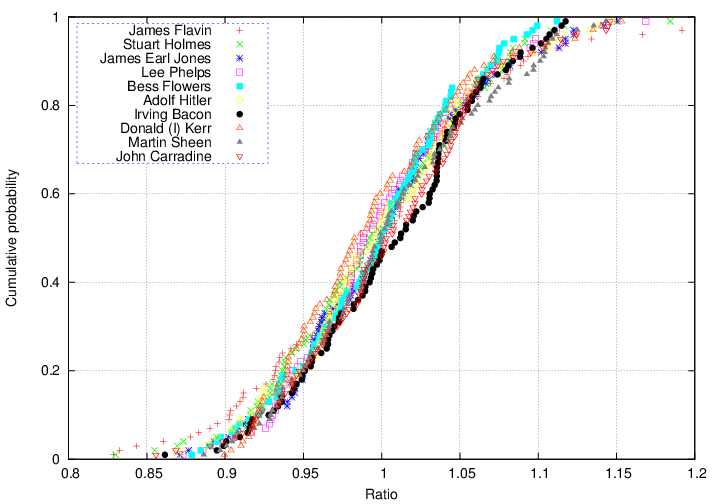
\includegraphics[width=1\textwidth]{plot256.png}
\caption{k=256}
\label{fig:exp256}
\end{figure}
\begin{figure}[h!]
\centering 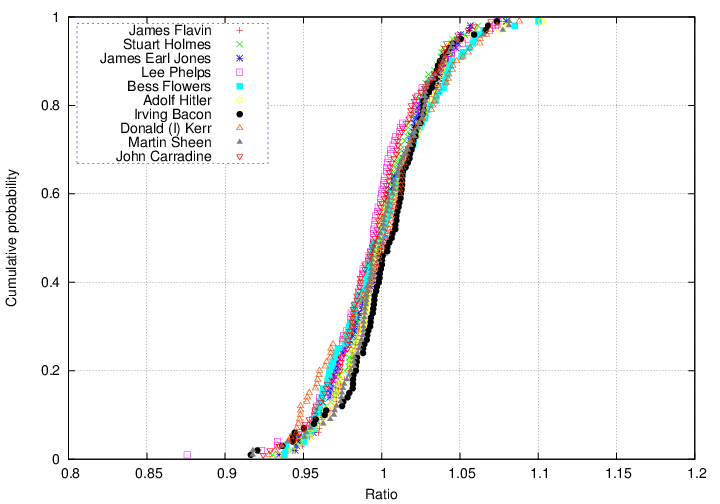
\includegraphics[width=1\textwidth]{plot1024.png}
\caption{k=1024}
\label{fig:exp1024}
\end{figure}
%explanation of experiments
%quality of approximation
  %valg af k
  %sammenhæng mellem k og sigma
  %eksperimentel validering af sammenhængen
  %estimaterne går i fløjten hvis k er for stor
  %sigma blir stor, hvis k er for lille
  %comparing results with part 1

\subsubsection{Suggested Improvements}
If $|W|<<n$ and the matrix is sparse, $|A_{\pi}|=1$ will occur often, Corresponding to iterating over a movie starring exactly one of the actors on the watchlist. In this case, the inner loop is poorly optimized. Firstly $p_i$ could be used, instead of $p_{max}$, and secondly it could be exploited that the values of $h(x_s, y_t)$ becomes smaller mod 1, when $t$ increases. Using a trick analogous to (TODO sbar while loop) could lower the bound on the inner loop from $O(p_{max}|A_i||C_i|)$ to $O(p|C_i|)$.

%do something about combine

\subsubsection{Conclusion}
We have presented an algorithm for approximating the size of boolean matrix products per row. The algorithm runs in linear time, if $p_{max}$ is chosen correctly. TODO delete this or talk about choosing $p_{max}$!.


%code in appendix

\section{Appendix}
\textbf{Popular.java - Map-Reduce}
\lstinputlisting[language=Java]{../map_reduce/popular/src/Popular.java}
\textbf{Popular.py - Project sql data into text file}
\lstinputlisting[language=Python]{../projections/popular.py}
\textbf{sequential\_popular.py - Sequential implementation of Popular}
\lstinputlisting[language=Python]{../tools/sequential_popular.py}
\textbf{sort\_and\_expand - Sort the output, and add actor names}
\lstinputlisting[language=Python]{../tools/sort_and_expand.py}


\end{document}
